\documentclass{article}
\usepackage{tikz}
\usetikzlibrary{calc}

\begin{document}

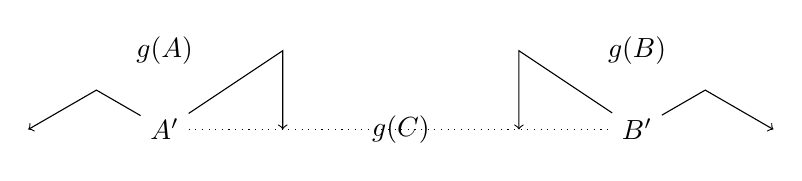
\begin{tikzpicture}[every node/.style={minimum width=0pt, minimum height=0pt}]
  % Define the coordinates of the nodes
  \node (A) at (-3,0) {$g(A)$};
  \node (B) at (3,0) {$g(B)$};
  \node (C) at (0,-1) {$g(C)$};
  \node (A') at ($(-3,-1)$) {$A'$};
  \node (B') at ($(3,-1)$) {$B'$};

  % Draw the lines from A', B' to A, B respectively
  \draw[->] (A') -- ++(150:1cm) -- ++(-150:1cm);
  \draw[->] (B') -- ++( 30:1cm) -- ++(-30:1cm);

  % Draw the dotted lines between A', B'
  \draw[dotted] (A') -- (B');
  
  % Draw the lines from A', B' to C
  \draw[->] (A') -- ($($(A')!0.5!(C)$)!1cm!90:(C)$) -- ($(A')!0.5!(C)$);
  \draw[->] (B') -- ($($(B')!0.5!(C)$)!1cm!-90:(C)$) -- ($(B')!0.5!(C)$);
\end{tikzpicture}

\begin{description}
  \item[Lowering the premises for a resolution inference in Case~2.] 
  The unlabeled leaves correspond to initial clauses from $f(\Gamma, h) \setminus \Gamma$, included earlier in $P_0$.
\end{description}

\end{document}